\documentclass[aspectratio=169,11pt]{beamer}

\usepackage{iftex}
\ifPDFTeX
  \usepackage[T1]{fontenc}
  \usepackage{helvet}
  \renewcommand{\familydefault}{\sfdefault}
\else
  \usepackage{fontspec}
  \setmainfont{texgyreheros-regular.otf}[BoldFont=texgyreheros-bold.otf,ItalicFont=texgyreheros-italic.otf,BoldItalicFont=texgyreheros-bolditalic.otf]
  \setsansfont{texgyreheros-regular.otf}[BoldFont=texgyreheros-bold.otf,ItalicFont=texgyreheros-italic.otf,BoldItalicFont=texgyreheros-bolditalic.otf]
  \setmonofont{texgyrecursor-regular.otf}[BoldFont=texgyrecursor-bold.otf,ItalicFont=texgyrecursor-italic.otf,BoldItalicFont=texgyrecursor-bolditalic.otf,Scale=MatchLowercase]
\fi
\usepackage[indonesian]{babel}
\usepackage{booktabs}
\usepackage{graphicx}
\usepackage{amsmath}
\usepackage{tikz}
\usetikzlibrary{positioning,arrows.meta,fit,backgrounds}

% ---------- palette and theme ----------
\definecolor{navy}{HTML}{1F3A5F}
\definecolor{accent}{HTML}{E4572E}
\definecolor{blu}{HTML}{4C78A8}
\definecolor{gry}{HTML}{6B7280}
\setbeamercolor{normal text}{fg=black!85}
\setbeamercolor{frametitle}{fg=navy}
\setbeamercolor{itemize item}{fg=accent}
\setbeamercolor{itemize subitem}{fg=accent}
\setbeamercolor{enumerate item}{fg=accent}
\setbeamertemplate{navigation symbols}{}
\setbeamertemplate{itemize item}[circle]
\setbeamertemplate{frametitle}{%
  \vspace{0.35cm}\par\noindent
  {\bfseries\large\color{navy}\insertframetitle\par}%
  \vspace{-0.15cm}{\color{accent}\rule{2.2cm}{2pt}}\par}
\setbeamertemplate{footline}{%
  \hfill{\scriptsize\color{gry}M. D. Nurkolis \;|\; Magister Informatika UII \;|\; \insertframenumber}\hspace{0.6cm}\vspace{0.3cm}}
\setbeamerfont{itemize/enumerate body}{size=\normalsize}

% card: width, colour, title, body
\newcommand{\card}[4]{%
  \begin{tikzpicture}[baseline=(card.north)]
    \node[draw=#2, line width=1.2pt, rounded corners=4pt, fill=#2!8,
          inner sep=8pt, anchor=north west] (card)
      {\begin{minipage}[t][3.1cm][t]{#1}\raggedright\hyphenpenalty=10000\exhyphenpenalty=10000
       {\bfseries\color{#2}#3}\par\vspace{4pt}#4\end{minipage}};
  \end{tikzpicture}}

\title{Prediksi Diabetes dengan Machine Learning tanpa Kebocoran Data}
\author{Mokhammad Dwi Nurkolis (NIM 26917015)}
\institute{Magister Informatika, Universitas Islam Indonesia}
\date{20 November 2026}

\begin{document}

% ---------- 1. Title ----------
\begin{frame}[plain]
  \vspace*{1.6cm}
  {\color{navy}\bfseries\LARGE Prediksi Diabetes dengan Machine Learning\\tanpa Kebocoran Data\par}
  \vspace{0.3cm}{\color{accent}\rule{3cm}{2.5pt}}\par\vspace{0.4cm}
  {\large Decision Tree, Random Forest, XGBoost, dan SVM pada dataset Pima Indians (768 pasien)\par}
  \vspace{1.0cm}
  {\bfseries Mokhammad Dwi Nurkolis} (NIM 26917015)\\
  Magister Informatika, Fakultas Teknologi Industri\\
  Universitas Islam Indonesia \;|\; 20 November 2026
\end{frame}

% ---------- 2. Problem ----------
\begin{frame}{Akurasi tinggi belum berarti aman untuk skrining diabetes}
  Studi sebelumnya pada dataset ini sering mengabaikan tiga hal:
  \vspace{0.4cm}

  \card{0.27\textwidth}{accent}{1. Nilai 0 yang mustahil}{Insulin bernilai 0 pada \textbf{48{,}7\%} pasien. Itu data hilang, bukan hasil ukur.}
  \hfill
  \card{0.27\textwidth}{blu}{2. Kelas tidak seimbang}{\textbf{65\%} sehat dan \textbf{35\%} diabetes. Model cenderung melewatkan pasien diabetes.}
  \hfill
  \card{0.27\textwidth}{navy}{3. Kebocoran data}{Imputasi atau SMOTE sebelum pembagian data membuat skor tampak lebih baik dari kenyataan.}
\end{frame}

% ---------- 3. Data ----------
\begin{frame}{Hampir separuh nilai insulin sebenarnya hilang}
  \begin{center}
    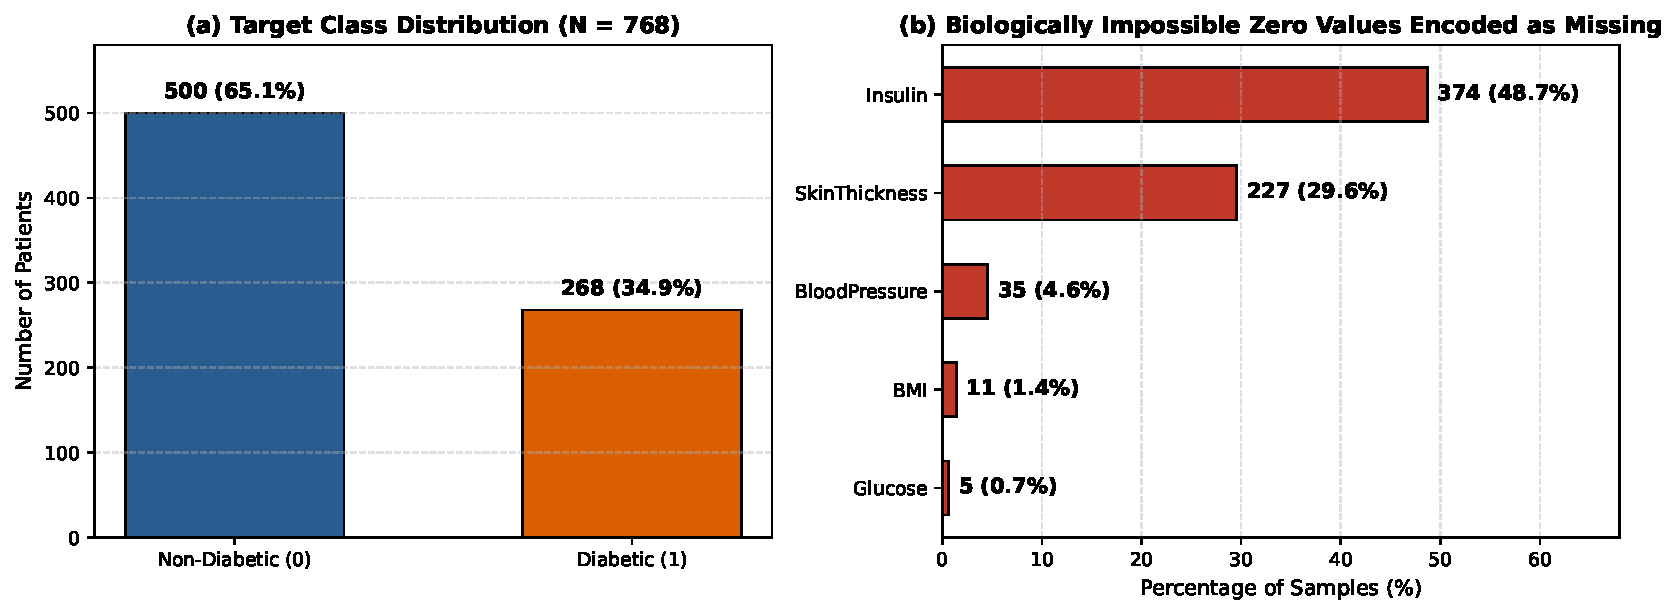
\includegraphics[height=0.58\textheight]{../artifacts/figures/fig1_class_and_missing_audit.pdf}
  \end{center}
  \vspace{-0.2cm}
  \begin{itemize}
    \item Nilai 0 pada lima fitur diubah menjadi \texttt{NaN}, lalu diisi \textbf{median} (distribusi miring ke kanan).
    \item Rata-rata insulin mentah 79,8; rata-rata nilai valid 155,6.
  \end{itemize}
\end{frame}

% ---------- 4. Pipeline ----------
\begin{frame}{Semua langkah dipelajari hanya dari data latih}
  \begin{itemize}
    \item Data dibagi \textbf{80:20} lebih dulu: 614 pasien latih, 154 pasien uji.
    \item Data uji tidak disentuh saat preprocessing maupun tuning.
  \end{itemize}
  \vspace{0.5cm}
  \begin{center}
  \begin{tikzpicture}[
      box/.style={draw=navy, fill=navy!8, rounded corners=3pt, minimum height=1.2cm,
                  minimum width=2.2cm, align=center, font=\small},
      arr/.style={-{Stealth}, thick, color=navy}]
    \node[box] (a) {Ubah\\0 $\to$ NaN};
    \node[box, right=0.4cm of a] (b) {Imputasi\\median};
    \node[box, right=0.4cm of b] (c) {Skala\\z-score};
    \node[box, right=0.4cm of c, fill=accent!15, draw=accent] (d) {SMOTE\\(hanya latih)};
    \node[box, right=0.4cm of d] (e) {Model};
    \draw[arr] (a)--(b); \draw[arr] (b)--(c); \draw[arr] (c)--(d); \draw[arr] (d)--(e);
    \begin{scope}[on background layer]
      \node[draw=gry, dashed, rounded corners=5pt, fit=(a)(e), inner sep=8pt,
            label={[font=\small, text=gry]above:di dalam setiap fold latih (CV 5-fold)}] {};
    \end{scope}
  \end{tikzpicture}
  \end{center}
  \vspace{0.3cm}
  Validasi dan pengujian memakai \textbf{data asli saja}; sampel sintetis tidak pernah muncul di sana.
\end{frame}

% ---------- 5. Design ----------
\begin{frame}{Tiga tahap eksperimen memisahkan pengaruh tiap perbaikan}
  \card{0.27\textwidth}{gry}{Exp. 1: Baseline}{Parameter bawaan.\\Tanpa SMOTE.}
  \hfill
  \card{0.27\textwidth}{blu}{Exp. 2: + SMOTE}{SMOTE di dalam fold latih.\\Parameter bawaan.}
  \hfill
  \card{0.27\textwidth}{accent}{Exp. 3: + Tuning}{SMOTE dan GridSearchCV 5-fold, dengan F1 sebagai target.}
  \vspace{0.5cm}

  Empat model: Decision Tree \;$\cdot$\; Random Forest \;$\cdot$\; XGBoost \;$\cdot$\; SVM (RBF)
\end{frame}

% ---------- 6. Result: sensitivity ----------
\begin{frame}{Sensitivity naik dari 0,48--0,61 menjadi 0,74--0,80}
  \begin{center}
    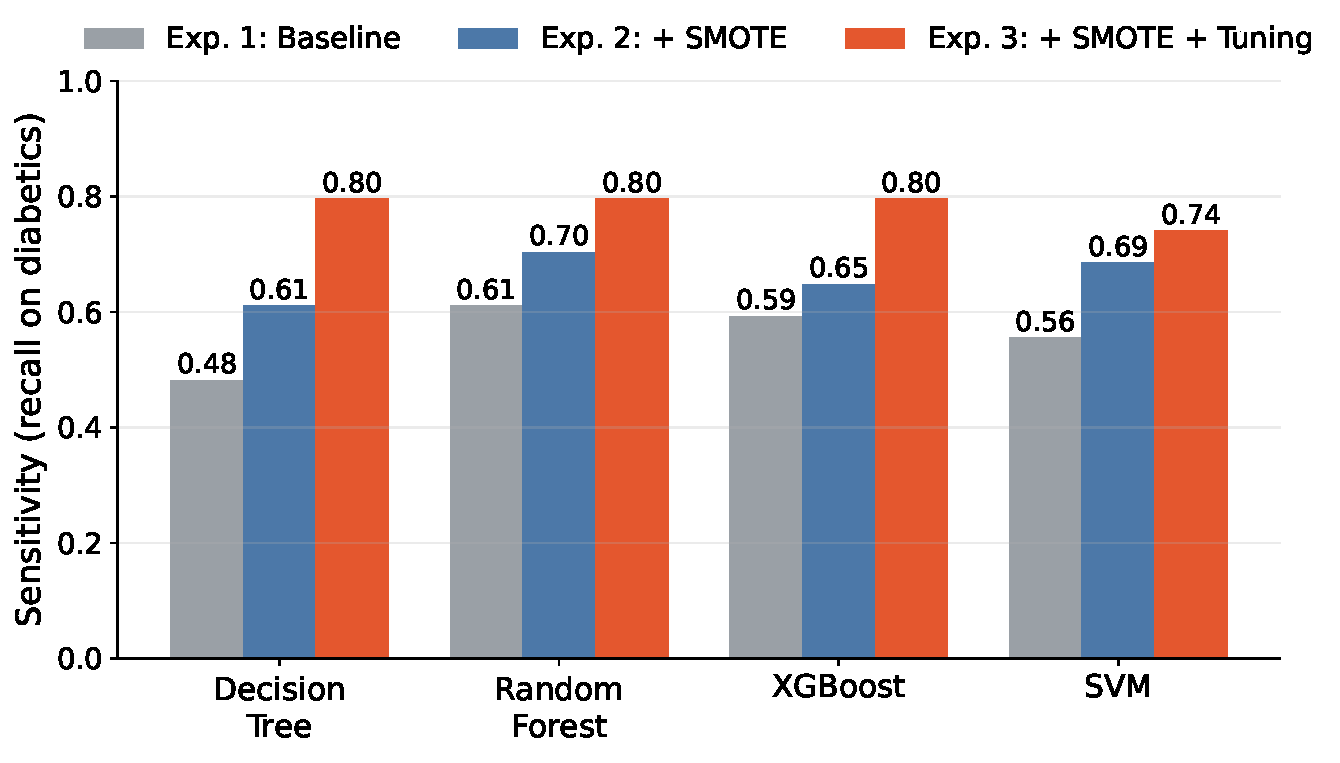
\includegraphics[height=0.66\textheight]{../artifacts/figures/slides/s_sensitivity_by_stage.pdf}
  \end{center}
  \vspace{-0.2cm}
  Hasil pada 154 pasien uji (54 diabetes). Spesifisitas turun dari 0,79--0,86 menjadi 0,70--0,75.
\end{frame}

% ---------- 7. Result: missed patients ----------
\begin{frame}{Pasien terlewat turun dari 28 menjadi 11 pada Decision Tree}
  \begin{center}
    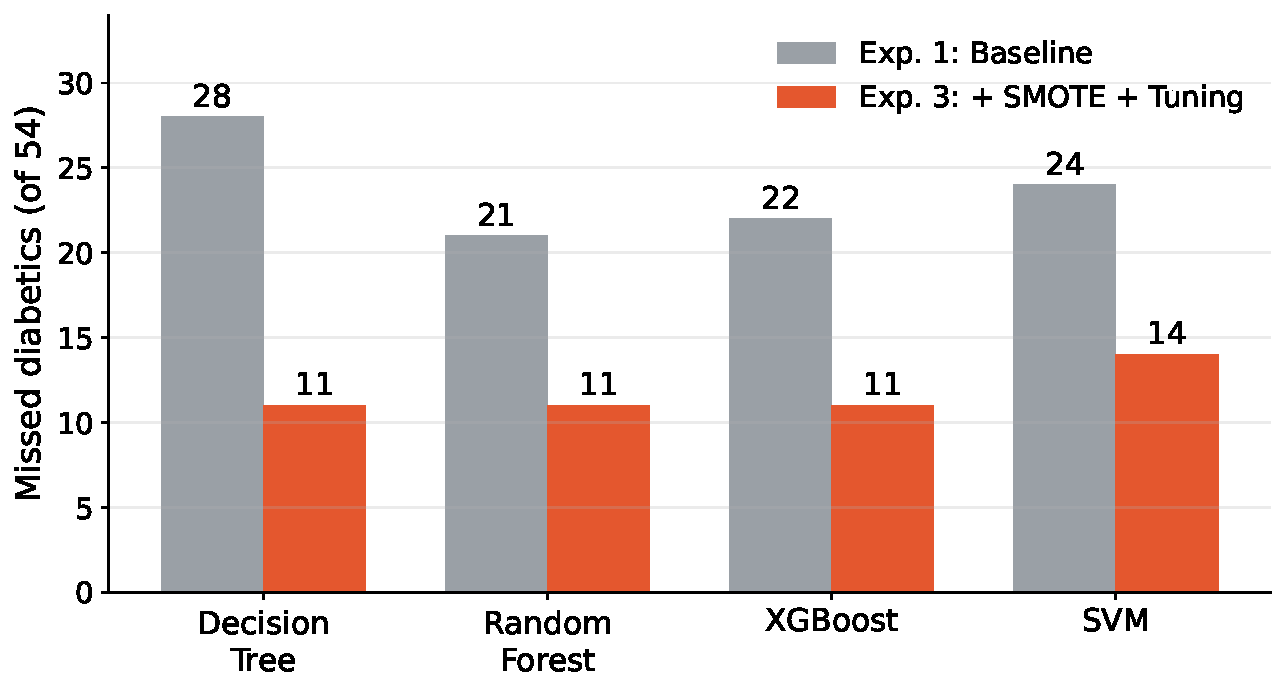
\includegraphics[height=0.66\textheight]{../artifacts/figures/slides/s_missed_patients.pdf}
  \end{center}
  \vspace{-0.2cm}
  Kesalahan yang paling berbahaya secara klinis, yaitu \emph{false negative}, berkurang pada semua model.
\end{frame}

% ---------- 8. Overfitting ----------
\begin{frame}{Regularisasi menekan overfitting pada model berbasis pohon}
  \begin{center}
    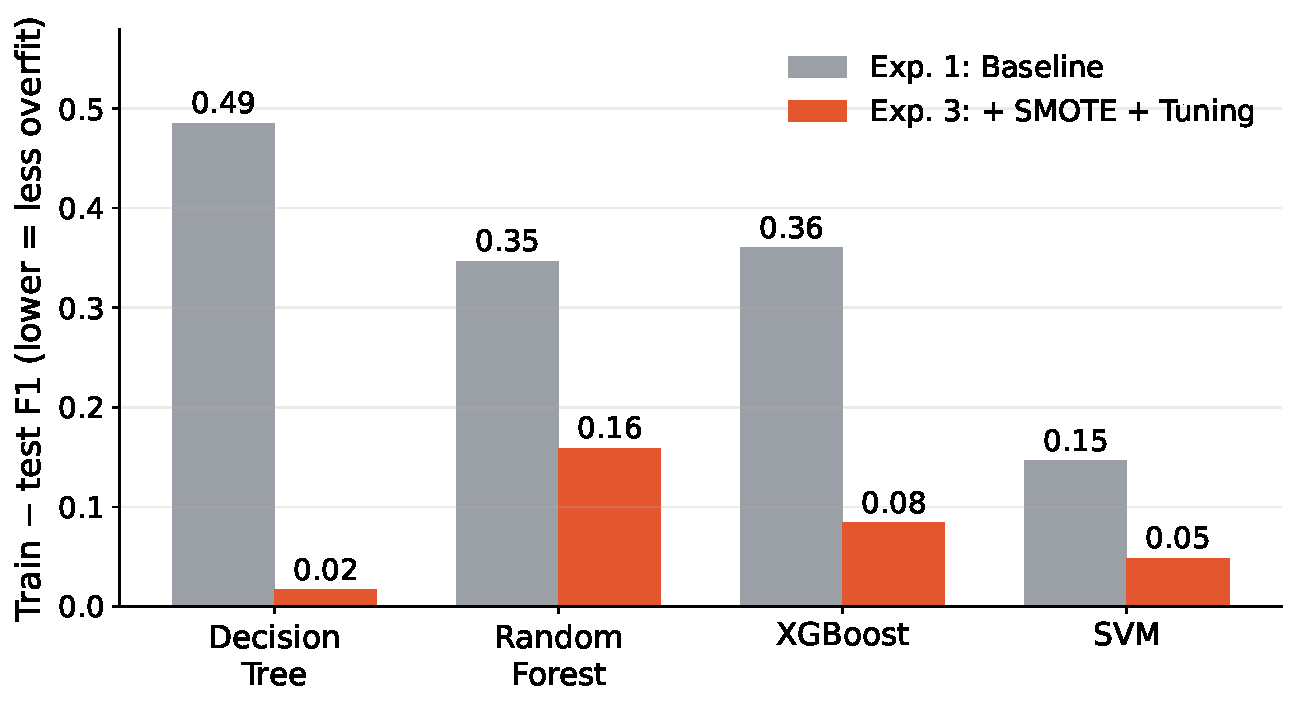
\includegraphics[height=0.62\textheight]{../artifacts/figures/slides/s_overfit_gap.pdf}
  \end{center}
  \vspace{-0.2cm}
  Tanpa pembatasan, F1 latih mencapai 1,00 pada pohon, forest, dan XGBoost. Setelah tuning, selisihnya 0,02--0,16.
\end{frame}

% ---------- 9. Model choice ----------
\begin{frame}{Model terbaik bergantung pada kebutuhan}
  \card{0.40\textwidth}{blu}{XGBoost: peringkat risiko}{ROC-AUC \textbf{0,818}, PR-AUC \textbf{0,708}.\\Sensitivity 0,796, CV F1 0,708, selisih train--test 0,084.}
  \hfill
  \card{0.40\textwidth}{accent}{Decision Tree (depth 4): aturan transparan}{F1 uji \textbf{0,705}, sensitivity 0,796, spesifisitas 0,750.\\Selisih train--test hanya 0,017.}
  \vspace{0.4cm}

  \textbf{Catatan:} data uji hanya memuat 54 pasien diabetes dan interval kepercayaan 95\% saling tumpang tindih. Perbedaan antarmodel tuned bersifat indikatif.
\end{frame}

% ---------- 10. Conclusion ----------
\begin{frame}{Kesimpulan}
  \begin{enumerate}
    \item Nilai 0 yang mustahil harus ditangani \textbf{di dalam} pipeline agar tidak ada kebocoran.
    \item Baseline tampak akurat (spesifisitas tinggi) tetapi melewatkan 39--52\% pasien diabetes.
    \item SMOTE di dalam fold dan tuning menaikkan sensitivity ke 0,74--0,80 dan menekan overfitting.
    \item Gunakan \textbf{XGBoost} untuk peringkat risiko dan \textbf{Decision Tree} untuk aturan yang mudah dijelaskan.
  \end{enumerate}
  \vspace{0.4cm}
  {\color{gry}\small Langkah berikutnya: nested CV, imputasi multivariat (MICE), kalibrasi probabilitas, dan validasi pada data multi-pusat.}
\end{frame}

% ---------- Backup ----------
\appendix

\begin{frame}{Cadangan: hasil Exp. 3 secara lengkap}
  \centering
  \small
  \begin{tabular}{lrrrrrrr}
    \toprule
    Model & CV F1 & Sens & Spec & F1 & ROC-AUC & PR-AUC & Selisih \\
    \midrule
    Decision Tree & 0,674 & \textbf{0,796} & \textbf{0,750} & \textbf{0,705} & 0,801 & 0,644 & \textbf{0,017} \\
    Random Forest & \textbf{0,711} & \textbf{0,796} & 0,700 & 0,677 & 0,815 & 0,697 & 0,159 \\
    XGBoost & 0,708 & \textbf{0,796} & 0,700 & 0,677 & \textbf{0,818} & \textbf{0,708} & 0,084 \\
    SVM (RBF) & 0,696 & 0,741 & 0,720 & 0,656 & 0,808 & 0,694 & 0,049 \\
    \bottomrule
  \end{tabular}

  \vspace{0.4cm}
  {\footnotesize Tebal = terbaik pada kolom. Selisih = F1 latih $-$ F1 uji. Tabel lengkap tiga tahap ada pada makalah.}
\end{frame}

\begin{frame}{Cadangan: kurva belajar (bias--variance)}
  \begin{center}
    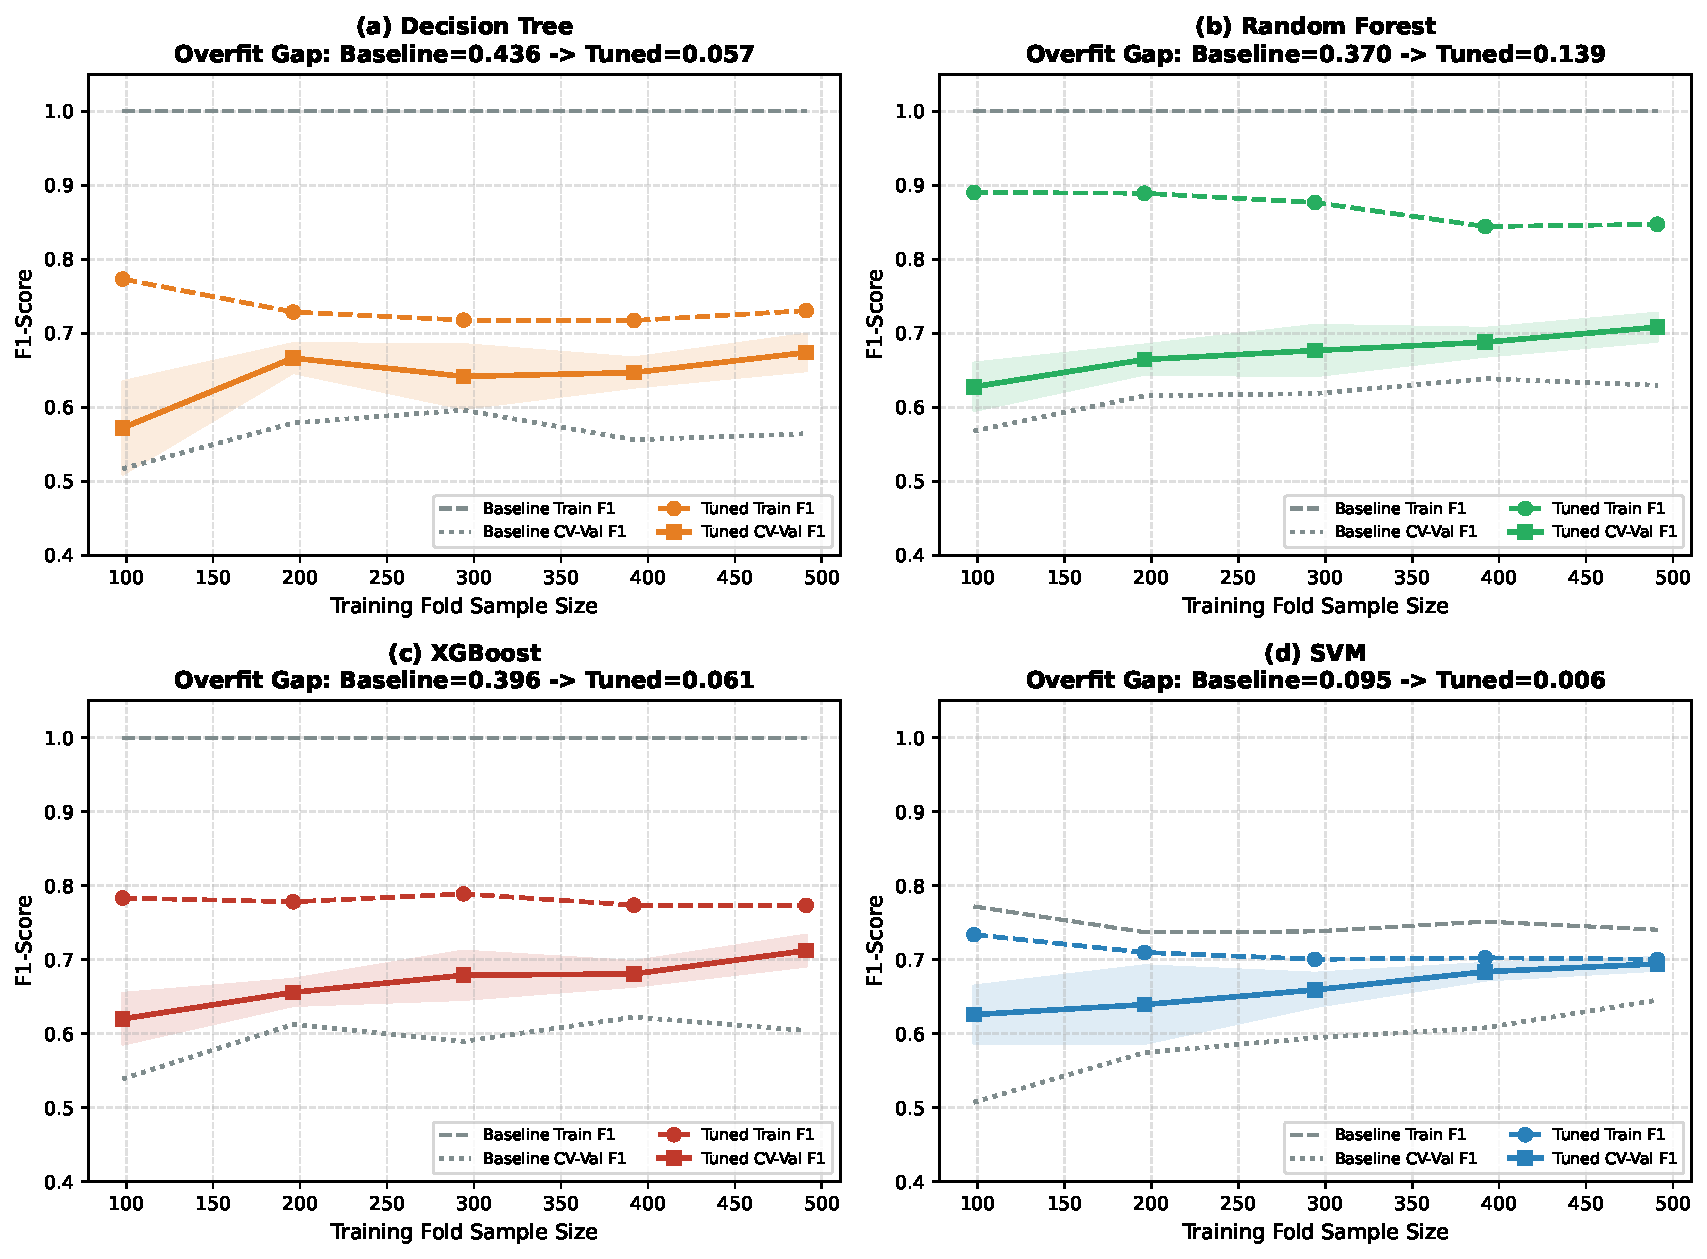
\includegraphics[height=0.74\textheight]{../artifacts/figures/fig5_learning_curves_bias_variance.pdf}
  \end{center}
\end{frame}

\begin{frame}{Cadangan: fitur yang paling berpengaruh}
  \begin{center}
    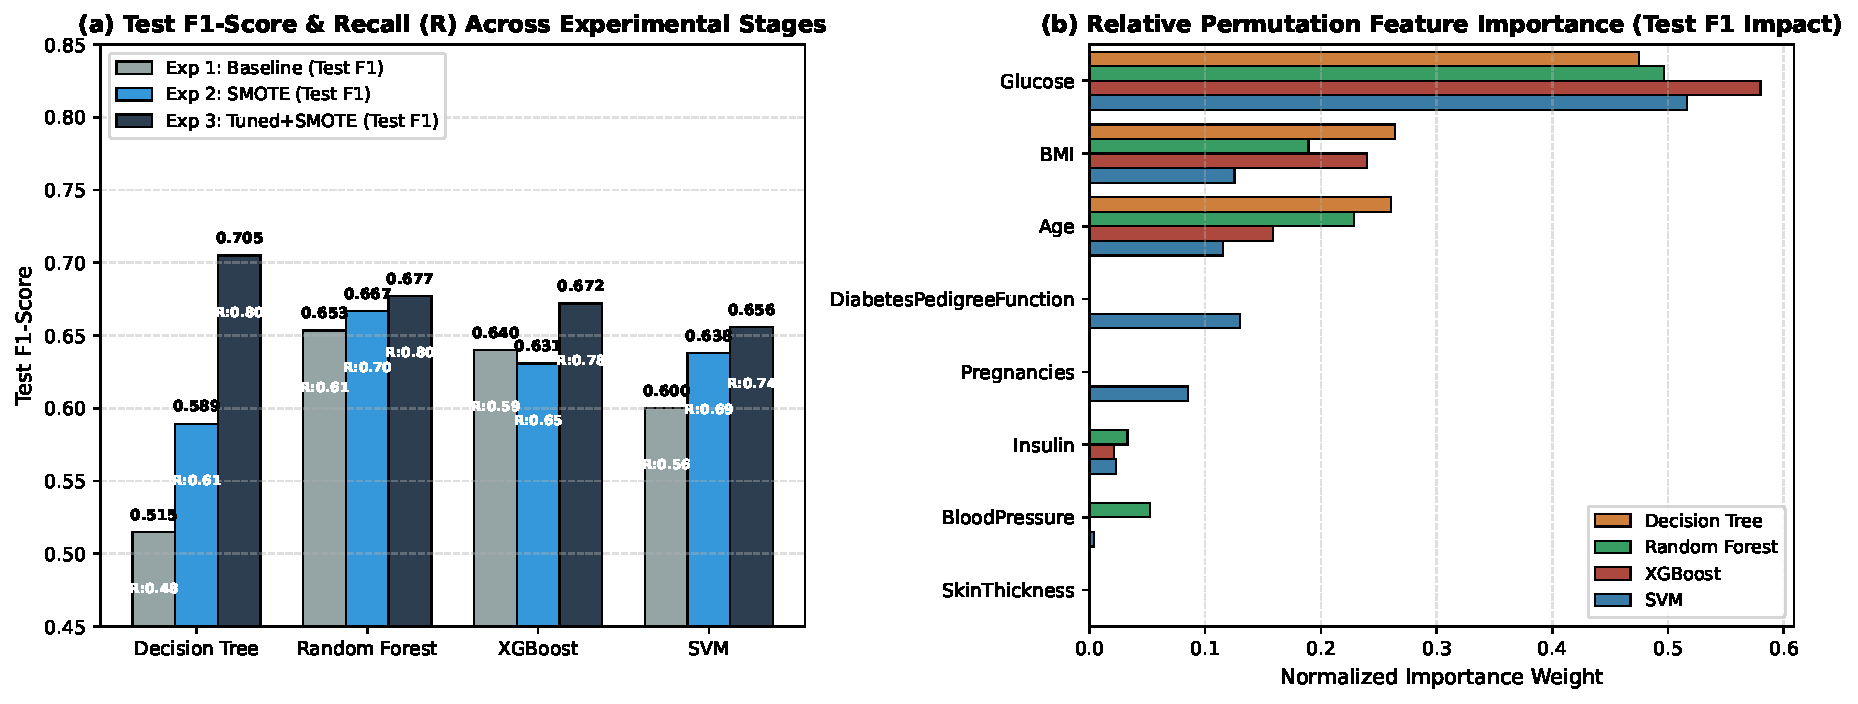
\includegraphics[width=0.92\textwidth]{../artifacts/figures/fig6_feature_importance.pdf}
  \end{center}
  Glucose, BMI, dan Age dominan pada semua model.
\end{frame}

\begin{frame}{Cadangan: confusion matrix model tuned}
  \begin{center}
    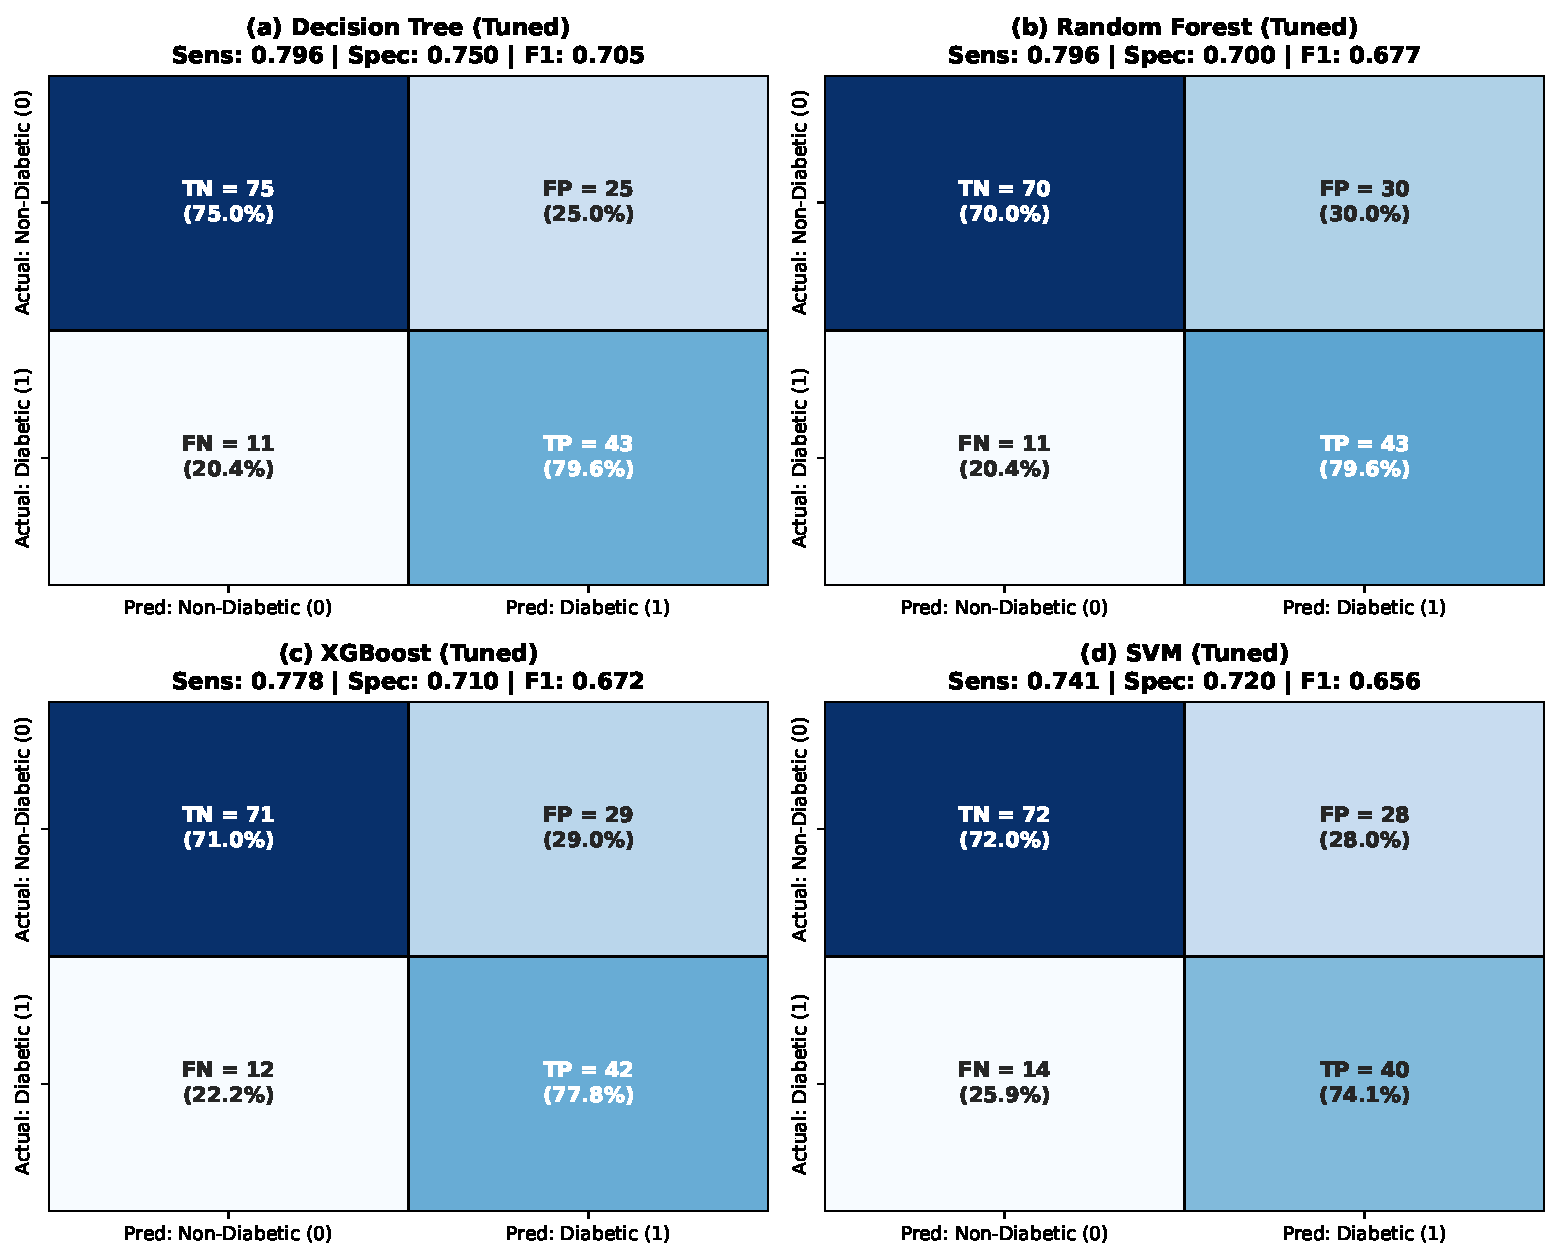
\includegraphics[height=0.74\textheight]{../artifacts/figures/fig3_confusion_matrices.pdf}
  \end{center}
\end{frame}

\end{document}
